\documentclass[11pt,a4paper]{article}

\usepackage[T1]{fontenc}
\usepackage[utf8]{inputenc}
\usepackage[margin=1in]{geometry}
\usepackage{hyperref}
\usepackage{xurl}
\usepackage{tabularx}
\usepackage{booktabs}
\usepackage{array}
\usepackage{xcolor}
\usepackage{float}
\usepackage{listings}
\usepackage{tikz}
\usepackage{titlesec}
\usetikzlibrary{arrows.meta,positioning,calc}
\emergencystretch=2em

\definecolor{boundgreen}{RGB}{223,242,216}
\definecolor{boundborder}{RGB}{76,140,74}
\definecolor{riskred}{RGB}{252,224,224}
\definecolor{riskborder}{RGB}{180,64,64}
\definecolor{flowblue}{RGB}{232,239,250}
\definecolor{flowborder}{RGB}{74,106,168}
\definecolor{statusgreen}{RGB}{223,242,216}
\newcommand{\statuschecked}{\texttt{checked}}
\newcommand{\statuspartial}{\texttt{partial}}
\newcommand{\statusnotyet}{\texttt{not yet}}
\newcommand{\statusna}{\texttt{n/a}}
\newcommand{\resultverified}{\colorbox{statusgreen}{\strut verified}}
\newcommand{\resultfalsified}{\colorbox{riskred}{\strut falsified}}
\newcommand{\resulttrue}{\colorbox{statusgreen}{\strut true}}
\newcommand{\resultfalse}{\colorbox{riskred}{\strut false}}
\newcommand{\resulttracefound}{\colorbox{riskred}{\strut trace found}}
\newcommand{\resultnotrace}{\colorbox{statusgreen}{\strut no trace found}}

\hypersetup{
  colorlinks=true,
  linkcolor=blue,
  urlcolor=blue,
  hypertexnames=false,
  pdftitle={A Machine-Checked Case Study Motivated by Recent Agent2Agent Discussion: Cocos AI aTLS},
  pdfauthor={Akira Okutomi}
}

\lstdefinestyle{shellstyle}{
  basicstyle=\ttfamily\small,
  breaklines=true,
  frame=single,
  columns=fullflexible
}

\title{A Machine-Checked Case Study Motivated by Recent Agent2Agent Discussion:\\Cocos AI aTLS}
\author{Akira Okutomi}
\date{April 12, 2026}

\begin{document}

\maketitle

\begin{abstract}
Motivated by the recent IETF agent2agent discussion about how to distinguish
informal security goals from machine-checked claims, this report presents a
small machine-checked case study of Cocos AI aTLS~\cite{cocosrepo}. In this
workspace, the current post-handshake design is analyzed through a layered
binding stack: live TLS session, channel-bound evidence, intended
infrastructure endpoint, intended agent or workload, intended task or
delegation context, and authorization. The strongest concrete finding is
exporter-label binding-parameter confusion in the current verifier path. A
second, weaker finding concerns policy-level handling when attestation is
explicitly required but no attestation extension is returned. The
same-endpoint results are reduced-model proof obligations: they separate
attested origin from stronger same-endpoint claims, but do not prove that the
complete RFC 9261 / Cocos post-handshake path is vulnerable. The workspace
combines implementation regression tests, Tamarin models, and
ProVerif~\cite{tamarin,proverif} models, with narrower checks for leaf-key
substitution, evidence/binder coupling, and session-scoped context reuse.
\end{abstract}

\section{Overview}

This report is framed as a machine-checked case study motivated by the recent
agent2agent discussion about protocol goals and machine-checked claims. Within
that framing, the workspace is centered on a small set of security questions
about attested origin, binding completeness, same-endpoint authenticity, and
agent-facing identity granularity. Its strongest implementation-facing result
is deliberately narrow: the current verifier accepts a self-declared
non-default exporter label instead of enforcing the locally expected Cocos
profile label. The report also records a weaker policy-level issue for
attestation-required flows that return no attestation extension. The
same-endpoint and L2--L4 identity/context results are treated separately as
reduced-model design obligations, not as demonstrated breaks of the complete
production post-handshake path.

The terminology is separated throughout the report. Relay-style same-endpoint
questions are treated as L0/L1 channel-binding questions. Diversion-style
questions are treated as L2 intended-infrastructure questions~\cite{idcrisis}.
Same-machine wrong-agent questions are treated as L3 agent or workload identity
questions. Task, thread, and delegation questions are treated as L4
application-context questions. The exporter-label issue is separate again: it
is binding-parameter confusion in the mechanism meant to bind attestation to
the TLS session, not a diversion or same-machine agent-identity claim.

Across the workspace, Go-language regressions act as implementation anchors for
concrete verifier behavior and are included under \path{verification/go-regressions/}.
Tamarin is used for request/offer gating,
attestation presence, expected-label enforcement, replay/one-shot behavior,
same-endpoint behavior under a reduced leakage model, and L2--L4
identity/context sketches.
ProVerif is used for correspondence-style clarification of attested origin vs.\
same-endpoint authenticity and the L2--L4 intended-subject obligations.

This workspace was also motivated by the IETF agent2agent mailing-list
discussion around how to separate informal security goals from smaller
machine-checked claims in protocol analysis~\cite{a2aml,fatt}.

The current workspace is organized around a small verification tree plus a
small set of implementation regressions.\footnote{Public artifact locations:
\path{verification/} and \path{verification/go-regressions/}. The Go-language
regressions run against a Cocos source checkout selected with
\texttt{COCOS\_SOURCE}.}

This report should not be read as a condemnation of Cocos AI or of the broader
goal of authenticated AI infrastructure. The project is attempting ambitious
work at the edge of current protocol and attestation practice, and that is
precisely why early machine-checked scrutiny is useful here. The intent of this
workspace is to make design assumptions and boundary conditions explicit while
the design is still evolving, not to dismiss the underlying direction.

\section{Scope}

This report focuses on the current post-handshake exported-authenticator form
introduced by Cocos AI through PR \#582 / commit \texttt{80bf813} (as of 9
April 2026)~\cite{cocos-pr582,cocos-80bf813}. The older intra-handshake design
is not the main subject of the report.

This report focuses on that current post-handshake aTLS behavior, while
examining same-endpoint behavior under the reduced A1 leakage assumption,
exporter-label binding-parameter handling, missing attestation after offer,
leaf-key substitution, L2--L4 intended-subject questions, and context reuse
through a mix of implementation tests and small formal models.

More concretely, it focuses on the exported-authenticator\footnote{In this
report, ``exported authenticator'' refers to the post-handshake TLS
authenticator exchange used by the current Cocos AI design, rather than a
certificate message carried inside the initial handshake~\cite{rfc9261}.} path used around
Cocos AI aTLS:

\begin{enumerate}
\item the client completes a TLS 1.3 handshake,
\item the client sends an exported-authenticator request with a fresh request
context,
\item the server constructs an authenticator and may attach CMW
attestation\footnote{In this report, ``CMW attestation'' refers to the
attestation payload and certificate-extension format used by the current Cocos
AI aTLS implementation.} data as a leaf extension,
\item the client validates the authenticator and then verifies the attestation
binder against the connection state, request context, and leaf public key.
\end{enumerate}

The modeling style is deliberately minimal. Each artifact aims to be a small
working model for one question at a time, rather than a single monolithic proof
attempt for the entire protocol stack.

The same-endpoint models abstract away many details of RFC 9261 and the Cocos
attestation-binder construction~\cite{rfc9261}, including the full
CertificateVerify and Finished transcript checks. They therefore ask a
narrower correspondence question:
whether the modeled attestation material and key possession imply that the
client's accepted peer is the exact live endpoint. They should not be read as
a claim that RFC 9261 exported authenticators, as a general mechanism, fail
under key leakage.

\section{Assumptions}

\begin{itemize}
\item The relay-style same-endpoint analysis uses an explicit A1 leakage
assumption: the attested leaf or ephemeral private key is revealed after
attestation issuance.
\item The current post-handshake relay models are abstraction checks over the
Cocos profile shape. They do not model the full RFC 9261
CertificateVerify/Finished validation path.
\item The context-reuse result is session-scoped: with
\texttt{ea.Session}\footnote{In this report, \texttt{ea.Session} refers to the
verifier-side state used to remember which request contexts have already been
accepted, so that the same context cannot be accepted twice.} the
workspace checks a one-shot guarantee; without session tracking, replay remains
possible at the API level.
\end{itemize}

\begin{table}[H]
\centering
\footnotesize
\begin{tabularx}{\textwidth}{@{}>{\raggedright\arraybackslash}p{0.15\textwidth}>{\raggedright\arraybackslash}p{0.33\textwidth}>{\raggedright\arraybackslash}X@{}}
\toprule
\textbf{Assumption} & \textbf{Meaning} & \textbf{Expected impact} \\
\midrule
A1 & Attested leaf or ephemeral private key leaks after attestation issuance. & Key possession may become transferable in the reduced model. A complete RFC 9261 / Cocos channel-binding path may still reject cross-channel use. \\
A2 & TLS exporter secret or application traffic secret leaks. & TLS session binding itself is compromised. This is stronger than A1 and is not the assumption used by the current reduced same-endpoint models. \\
A3 & Attestation signing key, reporting key, or attestation root material leaks. & The attestation trust root is compromised. This is outside the scope of this report. \\
\bottomrule
\end{tabularx}
\caption{Leakage assumptions separated for the report. The same-endpoint models use A1, not A2 or A3.}
\label{tab:leakage-assumptions}
\end{table}

\section{Out of Scope}

\begin{itemize}
\item A full symbolic model of TLS 1.3 or of the complete Cocos AI
implementation.
\item A claim that the complete RFC 9261 / Cocos post-handshake path is
vulnerable to same-endpoint failure.
\item End-to-end exploitability of the policy-level missing-attestation result
under the default server wiring.
\item Full diversion analysis beyond the minimal L2 infrastructure-identity
sketch included here.
\item Full X.509 certificate-chain validation and complete evidence-format
parsing.
\end{itemize}

\section{Binding Stack Used in This Report}

The report uses L0--L5 as the main organizing frame. Each layer asks which
subject must remain the same across the protocol boundary: the live TLS
session, the channel-bound evidence, the intended platform or deployment, the
intended agent or workload, the intended task context, or the intended
authorization. The lower layers concern TLS and attestation binding. The
higher layers concern Agent2Agent-style deployment and policy questions. This
L0--L5 notation is local to this report. It is not the same as Cocos
documentation that uses ``Level 2 Binding'' to describe TLS-session binding.

\begin{table}[H]
\centering
\footnotesize
\begin{tabularx}{\textwidth}{@{}>{\raggedright\arraybackslash}p{0.08\textwidth}>{\raggedright\arraybackslash}p{0.32\textwidth}>{\raggedright\arraybackslash}p{0.32\textwidth}>{\raggedright\arraybackslash}X@{}}
\toprule
\textbf{Layer} & \textbf{Question} & \textbf{Typical mechanism} & \textbf{Failure class} \\
\midrule
L0 & Is this the same live TLS session? & TLS 1.3 handshake, certificate validation, session keys, exporters. & MITM or session confusion. \\
L1 & Is the evidence or authenticator bound to that TLS session? & Exported Authenticators, TLS exporter binder, nonce, request context. & Relay, replay, borrowed evidence, binding-parameter confusion. \\
L2a & Is this the intended platform or VM? & Platform/VM evidence, measurement policy, and platform verifier output. & Diversion or wrong legitimate platform. \\
L2b & Is this the intended service, tenant, deployment, or environment? & Tenant, service, deployment, environment, host-data, or measurement-profile policy. & Diversion or wrong legitimate deployment. \\
L3 & Is this the intended agent, workload, or process? & Agent ID, workload ID, binary/config hash, agent key. & Same-machine wrong-agent. \\
L4 & Is this the intended task, thread, context, or delegation? & Task ID, thread ID, context ID, delegation token, callback binding. & Cross-thread or task confusion. \\
L5 & Is this action authorized for that agent and task? & Capability token, OAuth scope, policy engine, or user consent. & Confused deputy or privilege escalation. \\
\bottomrule
\end{tabularx}
\caption{Core binding stack used to organize the report. L2 is split into platform/VM appraisal and intended deployment identity because those are distinct checks in Cocos. A compact failure-class taxonomy is in Appendix~\ref{app:binding-taxonomy}.}
\label{tab:core-binding-stack}
\end{table}

The Tamarin and ProVerif models are then read against this stack. L1 checks
ask whether attested origin and key possession are enough for same-endpoint
authenticity. L2a checks ask whether a platform or VM is genuine and
policy-approved, while L2b asks whether that genuine platform is also the
intended tenant, service, deployment, or environment. L3 checks ask whether
machine-level attestation is enough for the intended agent. L4 checks ask
whether an agent-level acceptance is also tied to the intended task, thread, or
delegation context. L5 is noted
as an authorization and capability layer, but it is not modeled in this
workspace.

\section{Verification Artifacts and Implementation Flow}

The workspace is organized around three narrowly scoped security questions:

\begin{enumerate}
\item whether client acceptance preserves origin authenticity at the
attestation level,
\item what is explicitly bound into the attestation and binder inputs,
especially the request context, the leaf public key, and any TLS
exporter-derived values, and
\item whether client acceptance further establishes same-endpoint
authenticity, rather than only attested origin authenticity plus proof of
possession of the attested leaf key.
\end{enumerate}

The detailed code-path inventory and artifact layout are kept in the
verification README.\footnote{\path{verification/README.md}. For the current
design, the main moving parts are the internal transport request/response path,
the attestation provider, and the binder/verifier helpers under
\path{pkg/atls/}.}

\subsection{Current Post-Handshake Flow}

At the implementation level, the current Cocos AI flow relevant to this report is:

\begin{enumerate}
\item the client first completes a TLS 1.3 handshake,
\item the client builds an exported-authenticator request containing a fresh
context and the attestation offer extension,
\item the server receives that request and calls
\texttt{BuildLeafExtensions(...)} to construct the leaf certificate-entry
extensions for the authenticator response,
\item the default provider computes a binding from
\texttt{ExportKeyingMaterial(label, context)} and the leaf public key, then
embeds evidence plus binder values into a CMW attestation extension,
\item the client verifies the authenticator and, when the extension is present,
parses the attestation payload and verifies the binder.
\end{enumerate}

This is the execution path that the current verification artifacts try to
mirror.

\begin{figure}[H]
\centering
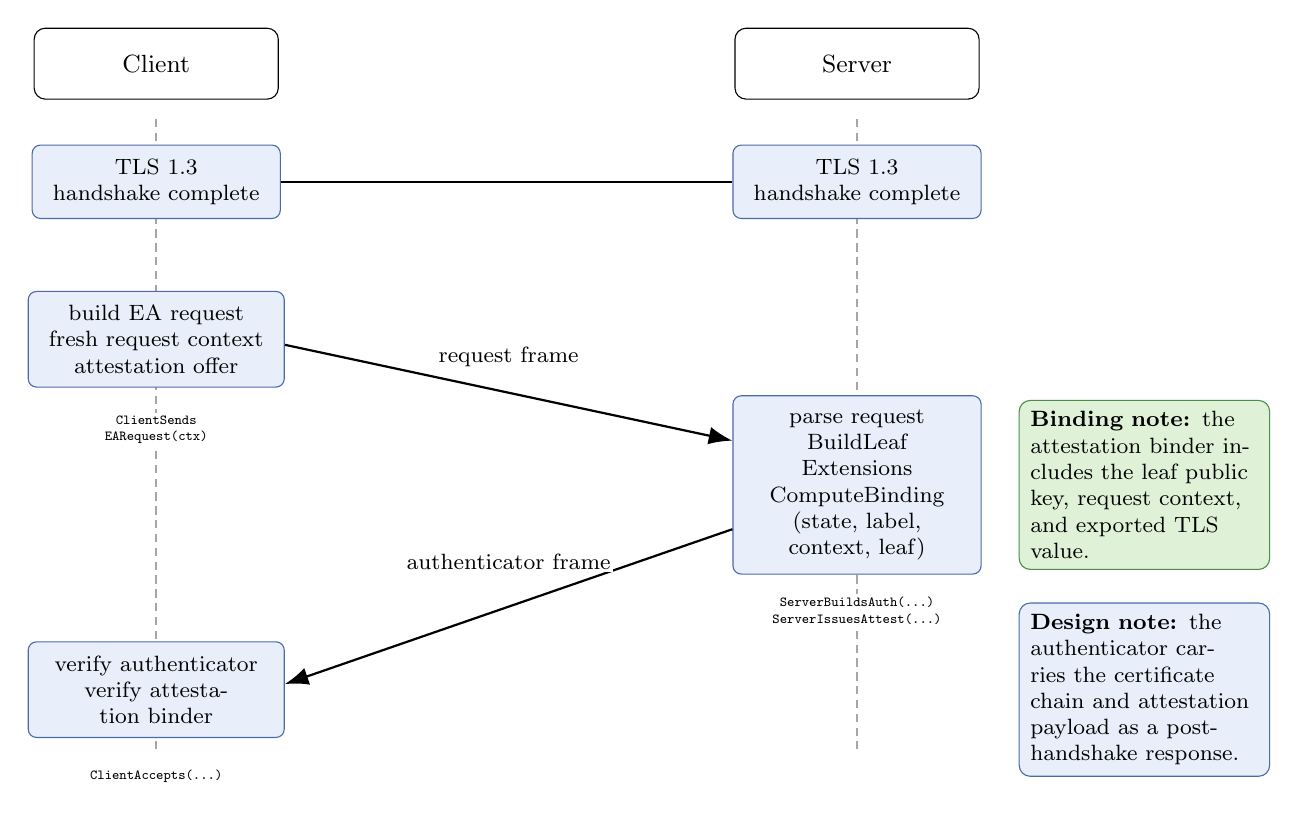
\begin{tikzpicture}[
  participant/.style={draw, rounded corners, minimum width=3.1cm, minimum height=0.9cm, align=center, font=\small},
  lifeline/.style={densely dashed, gray!70, thick},
  procbox/.style={draw=flowborder, fill=flowblue, rounded corners=3pt, align=center, font=\footnotesize, text width=2.8cm, inner sep=5pt},
  msg/.style={-{Latex[length=3mm]}, thick},
  msglabel/.style={font=\footnotesize, fill=white, inner sep=1pt, align=center},
  sidenote/.style={draw, rounded corners, align=left, font=\footnotesize, inner sep=4pt, text width=2.9cm},
  eventnote/.style={align=center, font=\tiny\ttfamily, text width=3.0cm, inner sep=1pt, fill=white},
  legend/.style={draw, rounded corners, font=\footnotesize, inner sep=3pt}
]
\node[participant] (client) at (0,0) {Client};
\node[participant] (server) at (8.9,0) {Server};

\draw[lifeline] (0,-0.7) -- (0,-8.7);
\draw[lifeline] (8.9,-0.7) -- (8.9,-8.7);

\node[procbox, text width=2.8cm] (curr_hs_c) at (0,-1.5) {TLS 1.3\\handshake complete};
\node[procbox, text width=2.8cm] (curr_hs_s) at (8.9,-1.5) {TLS 1.3\\handshake complete};

\draw[thick] (curr_hs_c.east) -- (curr_hs_s.west);

\node[procbox, text width=2.9cm] (curr_req) at (0,-3.5) {build EA request\\fresh request context\\attestation offer};
\node[eventnote] at (0,-4.65) {ClientSends\\EARequest(ctx)};

\node[procbox, text width=2.8cm] (curr_srv) at (8.9,-5.35) {parse request\\BuildLeaf\\Extensions\\ComputeBinding\\(state, label,\\context, leaf)};
\node[eventnote, text width=3.2cm] at (8.9,-6.95) {ServerBuildsAuth(...)\\ServerIssuesAttest(...)};

\draw[msg]
  ([yshift=-2pt]curr_req.east) --
  node[msglabel, above=8pt] {request frame}
  ([yshift=16pt]curr_srv.west);

\node[procbox, text width=2.9cm] (curr_verify) at (0,-7.95) {verify authenticator\\verify attestation binder};
\node[eventnote] at (0,-9.05) {ClientAccepts(...)};

\draw[msg]
  ([yshift=-16pt]curr_srv.west) --
  node[msglabel, above=12pt] {authenticator frame}
  ([yshift=2pt]curr_verify.east);

\node[sidenote, fill=boundgreen, draw=boundborder] at (12.55,-5.35)
  {\textbf{Binding note:} the attestation binder includes the leaf public key, request context, and exported TLS value.};
\node[sidenote, fill=flowblue, draw=flowborder] at (12.55,-7.95)
  {\textbf{Design note:} the authenticator carries the certificate chain and attestation payload as a post-handshake response.};
\end{tikzpicture}
\caption{Current post-handshake exported-authenticator flow, with simplified model-event anchors shown near the corresponding protocol points.}
\label{fig:current-flow}
\end{figure}

\section{Main Findings Summary}

\begin{table}[H]
\centering
\scriptsize
\renewcommand{\arraystretch}{1.18}
\begin{tabularx}{\textwidth}{@{}>{\raggedright\arraybackslash}p{0.21\textwidth}>{\raggedright\arraybackslash}p{0.24\textwidth}>{\raggedright\arraybackslash}p{0.18\textwidth}>{\raggedright\arraybackslash}X@{}}
\toprule
\textbf{Claim} & \textbf{Evidence} & \textbf{Strength} & \textbf{Vendor-facing action} \\
\midrule
Exporter-label binding-parameter confusion & Go regression + falsified Tamarin lemma + ProVerif correspondence & High & Enforce the locally expected Cocos exporter label and fail closed on mismatch. \\
Policy-level fail-open risk when attestation is explicitly required but no attestation extension is returned & Go regression + falsified Tamarin lemma & Medium & Distinguish a valid empty authenticator from \emph{attestation verified}; fail closed when attestation is required. \\
Evidence-to-binder coupling question & Go API-level harness & Medium / review item & Confirm that production evidence verification checks report data or challenge material against the recomputed TLS exporter binder. \\
Context replay outside explicit session tracking & Tamarin + API-level behavior & Medium & Require \texttt{ea.Session} or equivalent one-shot state for public validation paths that rely on fresh request contexts. \\
Reduced-model same-endpoint proof obligation & current ProVerif + current Tamarin attack trace\footnotemark & Low / exploratory & Model the full RFC 9261 CertificateVerify/Finished path, the Cocos exporter binder, and the exact leakage assumption before treating this as a production-path claim. \\
L2--L4 intended-subject obligations & Tamarin traces + ProVerif correspondences + bound sketches & Design obligation & Define how deployments bind intended infrastructure, agent/workload, and task/delegation context. This is not reported here as a Cocos production bug. \\
\bottomrule
\end{tabularx}
\renewcommand{\arraystretch}{1.0}
\caption{Claim strength summary for the current workspace. Implementation-facing claims are separated from reduced-model proof obligations and deployment-level design obligations.}
\label{tab:findings-summary}
\end{table}
\footnotetext{The same-endpoint models use A1 leakage from Table~\ref{tab:leakage-assumptions} and abstract away the full RFC 9261 CertificateVerify/Finished validation path.}

\vspace{0.5em}
Go-language regressions, Tamarin models, and ProVerif models play different
roles here rather than repeating the same check in three forms. The Go-language
tests anchor concrete verifier behavior in the current code path. Tamarin
captures gating, attestation presence, expected-label enforcement,
replay/one-shot behavior, and a same-endpoint trace under the reduced A1
leakage model.
ProVerif clarifies correspondence-style questions about attested origin,
same-endpoint authenticity, and L2--L4 intended-subject binding. A wider
Cocos snapshot and coverage note is included in Appendix~\ref{app:coverage}.

Across the current-design models, the machine-checked results should be read
layer by layer. At L1, the models separate attested origin from same-endpoint
authenticity and expose exporter-label binding-parameter confusion. At
L2--L4, the identity and task-context models are not implementation tests;
they show that platform/deployment identity, agent identity, and task context
are separate binding obligations.

\section{Current Design Results}

\subsection{Implementation Regression Tests (Go-language)}

The bundled Go-language regressions live in the public verification harness,
and are intended to mirror narrow current-design verifier behaviors from the
Cocos authenticator path.\footnote{\path{verification/go-regressions/}; related
Cocos source anchor: \path{pkg/atls/ea/authenticator_test.go}.} Their role here
is not to provide a formal security proof, but to act as implementation
anchors for several narrow security-relevant behaviors in the current code
path. In the report, the important point is what those tests check rather than
their exact names. The current set covers five behaviors:

\begin{itemize}
\item acceptance of a self-declared non-default exporter label during
attestation verification,
\item API-level acceptance when attestation is explicitly requested but the
authenticator carries no attestation extension,
\item API-level separation between evidence verification and binder
verification under a policy verifier that accepts the evidence bytes,
\item a narrow positive check against leaf-key substitution, and
\item the split between session-scoped one-shot context handling and replayable
API-level validation without session tracking.
\end{itemize}

The focused Go regression harness is bundled in the verification tree and runs
against a Cocos source checkout.\footnote{\path{verification/go-regressions/}}

\subsection{Tamarin Results}

The current-design Tamarin artifacts are summarized in the Tamarin
README.\footnote{\path{verification/post-handshake/README.md}} Together they cover
attestation offer vs.\ plain request, authenticator origin, attestation
presence, exporter-label binding-parameter enforcement, one-shot vs.\ replayable
request-context usage, abstract L2 infrastructure identity, same-machine
agent identity, and L4 task/context binding. The infrastructure, agent, and
task/context rows in
Table~\ref{tab:tamarin-results} are narrow identity sketches, not relay models.

\begin{table}[H]
\centering
\scriptsize
\begin{tabularx}{\textwidth}{@{}>{\raggedright\arraybackslash}p{0.27\textwidth}>{\raggedright\arraybackslash}X>{\raggedright\arraybackslash}p{0.18\textwidth}@{}}
\toprule
\textbf{Property} & \textbf{Meaning} & \textbf{Result} \\
\midrule
(1) Server-origin authenticity & An attested client acceptance must correspond to a server-side authenticator creation event. & \resultverified \\
(2) Offer-gated acceptance & A successful acceptance must be preceded by a client attestation offer. & \resultverified \\
(3) No attested acceptance from plain mode & Plain requests do not lead to attested acceptance. & \resultverified \\
(4) Exporter-label binding-parameter enforcement & Accepted attestations should only use the expected Cocos profile label. & \resultfalsified \\
(5) No success without required attestation & An attestation-required request should not report success when the attestation extension is missing. & \resultfalsified \\
(6) Reduced-model same-endpoint trace under A1 leakage & In a model that omits the full RFC 9261 CertificateVerify/Finished path, there exists a client-accepted session that does not establish same-endpoint authenticity. & \resulttracefound \\
(7) Session-scoped one-shot context use & With explicit session tracking, the same request context cannot be accepted twice. & \resultverified \\
(8) Replay without session tracking & Without session tracking, there exists a replay trace for the same request context. & \resulttracefound \\
(9) Diversion trace with shared measurement & A client acceptance of the intended infrastructure endpoint can be satisfied by another genuine endpoint with the same measurement. & \resulttracefound \\
(10) Diversion trace under intended-infrastructure-bound mitigation & Under the intended-infrastructure-bound sketch, that direct diversion trace is no longer found. & \resultnotrace \\
(11) Wrong-agent trace on the same machine & A client acceptance of the intended agent can still be satisfied by another co-resident agent on the same attested machine. & \resulttracefound \\
(12) Wrong-agent trace under intended-agent-bound mitigation & Under the intended-agent-bound sketch, that same-machine wrong-agent trace is no longer found. & \resultnotrace \\
(13) Wrong-task trace under the same agent & A client acceptance for the intended task can still be satisfied by another task/thread/delegation context served by the same agent. & \resulttracefound \\
(14) Wrong-task trace under intended-task-bound mitigation & Under the intended-task-bound sketch, that direct wrong-task trace is no longer found. & \resultnotrace \\
\bottomrule
\end{tabularx}
\caption{Summary of current-design Tamarin results.}
\label{tab:tamarin-results}
\end{table}
{\footnotesize\raggedright File mapping under
\texttt{verification/post-handshake/tamarin/}: (1)--(5)
\texttt{cocos\_attestation.spthy}; (6)
\texttt{cocos\_same\_endpoint\_current.spthy}; (7)--(8)
\texttt{cocos\_context\_reuse\_current.spthy}; (9)
\texttt{cocos\_infrastructure\_identity\_current.spthy}; (10)
\texttt{cocos\_infrastructure\_identity\_bound\_current.spthy}; (11)
\texttt{cocos\_agent\_identity\_current.spthy}; (12)
\texttt{cocos\_agent\_identity\_bound\_current.spthy}; (13)
\texttt{cocos\_task\_context\_current.spthy}; (14)
\texttt{cocos\_task\_context\_bound\_current.spthy}.\par}

The falsified expected-label lemma is the stronger additional finding. The
falsified missing-required-attestation lemma is weaker because its reachability
in the default server wiring has not been shown end-to-end.

A separate current-design Tamarin model checks a reduced same-endpoint
correspondence under the A1 leakage assumption.\footnote{\path{verification/post-handshake/tamarin/cocos_same_endpoint_current.spthy}}
In that model:
\begin{itemize}
\item \texttt{received\_attestation\_has\_server\_origin} is verified,
\item \texttt{same\_endpoint\_can\_fail\_under\_leakage} has a verified attack
trace.
\end{itemize}
This mirrors the relay/same-endpoint split also seen in the ProVerif artifacts,
but it remains a reduced-model signal rather than a claim about the complete
RFC 9261 / Cocos validation path.

A separate session-scoped Tamarin model checks a different
question.\footnote{\path{verification/post-handshake/tamarin/cocos_context_reuse_current.spthy}}
In that model,
\texttt{session\_context\_is\_one\_shot} is verified and
\texttt{no\_session\_replay\_exists} has a verified replay trace. This is meant
to track the semantics of \texttt{ea.Session}; it should not be read as a claim
that every current-design validation path is automatically one-shot.

A second pair of current-design Tamarin models checks an abstract L2
diversion-style identity question: whether a valid shared measurement is enough
to identify the intended infrastructure endpoint.\footnote{\path{verification/post-handshake/tamarin/cocos_infrastructure_identity_current.spthy};
\path{verification/post-handshake/tamarin/cocos_infrastructure_identity_bound_current.spthy}}
The unbound model verifies valid-measurement origin and yields a trace where
another genuine infrastructure endpoint with the same measurement satisfies a
client acceptance for the intended infrastructure identity. The mitigation
sketch verifies intended-infrastructure origin and response, and the direct
diversion trace is no longer found. This is still a narrow model, but it is
now a machine-checked L2 sketch rather than only a taxonomy entry. It does not
model concrete evidence fields, CoRIM policy semantics, or deployment identity
sources.

A third pair of current-design Tamarin models checks a different identity
gap: whether machine-level attestation can distinguish the intended AI agent
from another co-resident agent on the same attested machine.\footnote{\path{verification/post-handshake/tamarin/cocos_agent_identity_current.spthy};
\path{verification/post-handshake/tamarin/cocos_agent_identity_bound_current.spthy}}
The unbound model verifies machine origin and yields a wrong-agent attack
trace on the same machine. The mitigation sketch also verifies machine origin,
but the same wrong-agent trace is no longer found. This remains a narrow
design sketch, but in this abstraction it shows that binding both the
attestation and the live response to the intended agent removes the
co-resident-agent confusion trace.

A fourth pair of current-design Tamarin models checks the L4 task/context
question: whether a valid response from the intended agent is also tied to the
intended task, thread, or delegation context.\footnote{\path{verification/post-handshake/tamarin/cocos_task_context_current.spthy};
\path{verification/post-handshake/tamarin/cocos_task_context_bound_current.spthy}}
The unbound model verifies agent-level attestation origin and yields a
wrong-task trace under the same agent. The mitigation sketch binds the task
identity into the attestation and response shape; in that abstraction, the
direct wrong-task trace is no longer found.

\subsection{ProVerif Results}

The ProVerif artifacts are summarized in the ProVerif
README.\footnote{\path{verification/post-handshake/README.md}} They were added
to express the main current-design questions as correspondence queries:
attested origin vs.\ same-endpoint authenticity, expected exporter-label use,
leaf-key substitution resistance, and L2--L4 intended-subject binding.

The attack assumption behind the same-endpoint models is A1 from
Table~\ref{tab:leakage-assumptions}: leakage of the attested leaf or ephemeral
private key after attestation issuance. The models do not assume leakage of
TLS exporter secrets or attestation root keys.

\begin{table}[H]
\centering
\scriptsize
\begin{tabularx}{\textwidth}{@{}>{\raggedright\arraybackslash}p{0.31\textwidth}>{\raggedright\arraybackslash}X@{}}
\toprule
\textbf{Model event} & \textbf{Protocol point represented} \\
\midrule
\path{ClientSendsEARequest(ctx)} & The client sends an exported-authenticator request with a fresh request context. \\
\path{ServerBuildsAuthenticator(channel,ctx,leaf)} & The server constructs the authenticator for a request, channel name, and leaf key in the model. \\
\path{ServerIssuesAttestation(binding)} & The model records genuine server-side attestation origin for the attestation material. \\
\path{ClientAccepts(ctx,leaf,label)} & The client accepts the authenticator after verifier-side checks in the model. \\
\path{ServerBindsSameChannel(channel)} & The honest server answers the client's live-channel challenge on the same modeled channel. \\
\bottomrule
\end{tabularx}
\caption{Event-to-query mapping for the current post-handshake ProVerif/Tamarin flow. The arities are simplified for readability; exact arguments are in the model files.}
\label{tab:event-mapping}
\end{table}

\subsubsection*{Current-Design Results}

\begin{table}[H]
\centering
\footnotesize
\begin{tabularx}{\textwidth}{@{}>{\raggedright\arraybackslash}p{0.20\textwidth}>{\raggedright\arraybackslash}p{0.34\textwidth}>{\centering\arraybackslash}p{0.11\textwidth}>{\raggedright\arraybackslash}X@{}}
\toprule
\textbf{Model thread} & \textbf{Correspondence query} & \textbf{Result} & \textbf{Interpretation} \\
\midrule
(1) Request-gated acceptance &
\texttt{ClientAccepts ==> ClientSendsEARequest} &
\resulttrue{} &
Acceptance still implies a prior client-side exported-authenticator request. \\
(2) Server-side attestation origin &
\texttt{ClientAccepts ==> ServerIssuesAttestation} &
\resulttrue{} &
Client acceptance still tracks genuine server-side attestation origin. \\
(3) Server-side binding/construction event &
\texttt{ClientAccepts ==> ServerBuildsAuthenticator} &
\resultfalse{} &
Under A1 leakage, the reduced relay model does not preserve the same server-side build event. \\
(4) Relay / same-endpoint authenticity &
\texttt{current: ClientAccepts ==> ServerBindsSameChannel} &
\resultfalse{} &
Under A1 leakage, the reduced relay model does not establish same-endpoint authenticity. \\
(5) Expected Cocos exporter-label enforcement &
\texttt{current: ClientAccepts ==> ServerUsesDefaultLabel} &
\resultfalse{} &
Acceptance does not imply use of the expected Cocos profile label. \\
(6) Leaf-key substitution resistance &
\texttt{current: ClientAccepts ==> ServerAttestsLeafKey} &
\resulttrue{} &
Client acceptance remains tied to the attested leaf public key. \\
\bottomrule
\end{tabularx}
\caption{Summary of current-design ProVerif correspondence queries for channel binding and verifier behavior.}
\label{tab:proverif-results}
\end{table}

\begin{table}[H]
\centering
\footnotesize
\begin{tabularx}{\textwidth}{@{}>{\raggedright\arraybackslash}p{0.20\textwidth}>{\raggedright\arraybackslash}p{0.34\textwidth}>{\centering\arraybackslash}p{0.11\textwidth}>{\raggedright\arraybackslash}X@{}}
\toprule
\textbf{Model thread} & \textbf{Correspondence query} & \textbf{Result} & \textbf{Interpretation} \\
\midrule
(7) L2 infrastructure identity &
\texttt{AcceptsInfra ==> MeasurementIssued} &
\resulttrue{} &
Acceptance still implies a valid shared-measurement attestation. \\
(8) L2 intended-infrastructure endpoint &
\texttt{AcceptsInfra ==> IntendedInfraResponded} &
\resultfalse{} &
Without intended-infrastructure binding, another genuine endpoint with the same measurement can satisfy acceptance. \\
(9) L2 intended-infrastructure-bound sketch &
\texttt{AcceptsInfra ==> IntendedInfraResponded} &
\resulttrue{} &
When the intended infrastructure identity is part of the signed attestation consumed by the client, the modeled diversion-style correspondence holds. \\
(10) L3 machine-level attestation vs.\ intended agent &
\texttt{AcceptsAgent ==> MachineAttestationIssued} &
\resulttrue{} &
Acceptance still implies valid machine-level attestation. \\
(11) L3 intended-agent response &
\texttt{AcceptsAgent ==> IntendedAgentResponded} &
\resultfalse{} &
Without intended-agent binding, another co-resident agent on the same attested machine can satisfy acceptance. \\
(12) L3 intended-agent-bound sketch &
\texttt{AcceptsAgent ==> IntendedAgentResponded} &
\resulttrue{} &
When the intended agent identity is part of the signed attestation consumed by the client, the modeled wrong-agent correspondence holds. \\
(13) L4 agent-level attestation vs.\ intended task &
\texttt{AcceptsTask ==> AgentAttestationIssued} &
\resulttrue{} &
Acceptance still implies valid agent-level attestation. \\
(14) L4 intended-task response &
\texttt{AcceptsTask ==> IntendedTaskResponded} &
\resultfalse{} &
Without intended-task binding, another task/thread/delegation context served by the same agent can satisfy acceptance. \\
(15) L4 intended-task-bound sketch &
\texttt{AcceptsTask ==> IntendedTaskResponded} &
\resulttrue{} &
When the intended task identity is part of the signed attestation and live response consumed by the client, the modeled task-context correspondence holds. \\
\bottomrule
\end{tabularx}
\caption{Summary of current-design ProVerif correspondence queries for identity and task/context binding sketches.}
\label{tab:proverif-identity-results}
\end{table}
{\footnotesize\raggedright File mapping under
\texttt{verification/post-handshake/proverif/}: (1)--(4)
\texttt{cocos\_relay\_attack.pv}; (5)
\texttt{cocos\_exporter\_label\_current.pv}; (6)
\texttt{cocos\_leaf\_key\_substitution\_current.pv}; (7)--(8)
\texttt{cocos\_infrastructure\_identity\_current.pv}; (9)
\texttt{cocos\_infrastructure\_identity\_bound\_current.pv}; (10)--(11)
\texttt{cocos\_agent\_identity\_current.pv}; (12)
\texttt{cocos\_agent\_identity\_bound\_current.pv}; (13)--(14)
\texttt{cocos\_task\_context\_current.pv}; (15)
\texttt{cocos\_task\_context\_bound\_current.pv}.\par}

Taken together with the other checks, the ProVerif side gives a narrower
binding picture for the current design: it supports binding to the request
context and leaf key. Under the reduced abstraction used by the relay models,
it does not prove that the client's live peer is the same endpoint that
produced the server-side attestation material. This leaves same-endpoint
authenticity as a model-completeness and proof obligation. It is not evidence
that the complete RFC 9261 / Cocos post-handshake path fails under key leakage.

Figure~\ref{fig:relay} gives the relay-style same-endpoint intuition behind those
current-design ProVerif results and highlights the gap between attested origin
and same-endpoint authenticity.

\begin{figure}[H]
\centering
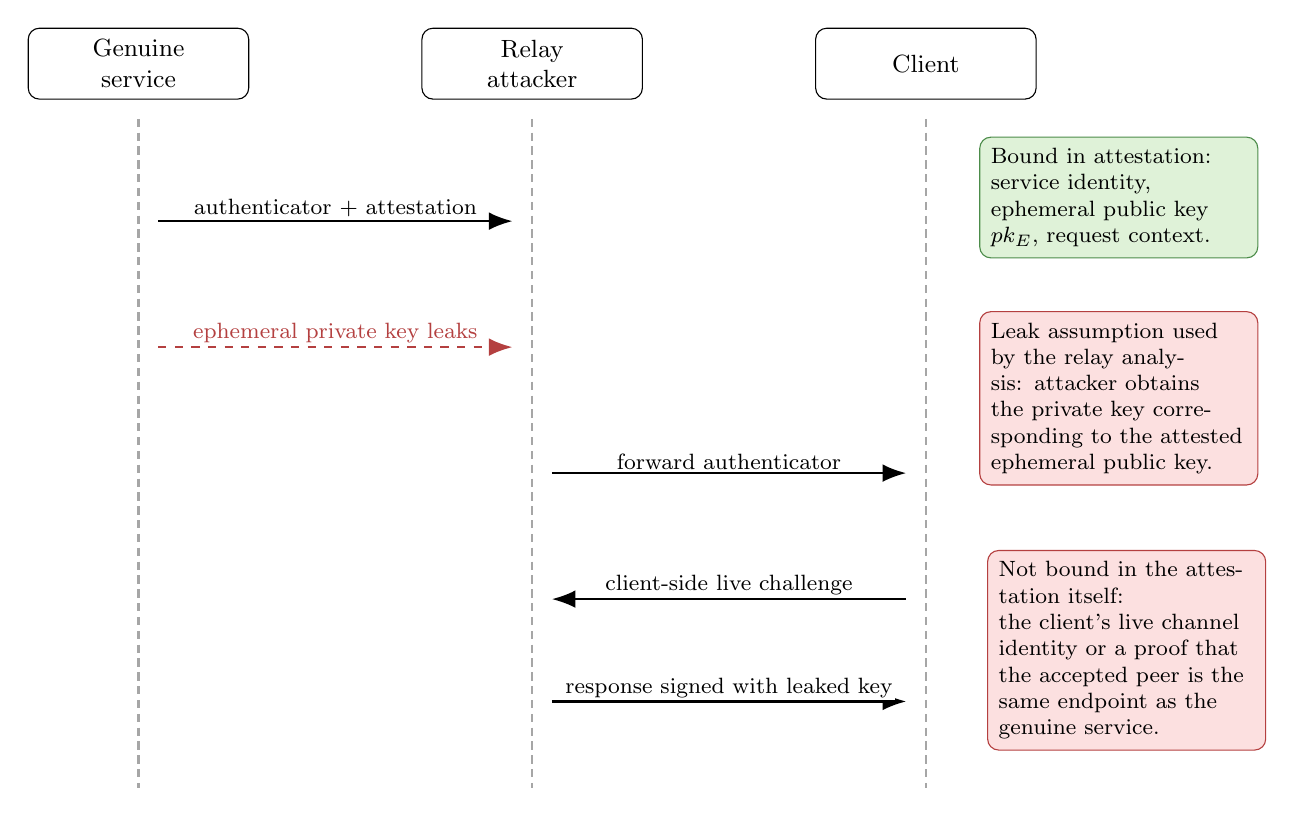
\begin{tikzpicture}[
  participant/.style={draw, rounded corners, minimum width=2.8cm, minimum height=0.9cm, align=center, font=\small},
  lifeline/.style={densely dashed, gray!70, thick},
  msg/.style={-{Latex[length=3mm]}, thick},
  leak/.style={-{Latex[length=3mm]}, thick, dashed, riskborder},
  msglabel/.style={font=\footnotesize, fill=white, inner sep=1pt, align=center},
  sidenote/.style={draw, rounded corners, align=left, font=\footnotesize, inner sep=4pt, text width=3.25cm},
  legend/.style={draw, rounded corners, font=\footnotesize, inner sep=3pt}
]
\node[participant] (svc) at (0,0) {Genuine\\service};
\node[participant] (att) at (5.0,0) {Relay\\attacker};
\node[participant] (cli) at (10.0,0) {Client};

\draw[lifeline] (0,-0.7) -- (0,-9.2);
\draw[lifeline] (5.0,-0.7) -- (5.0,-9.2);
\draw[lifeline] (10.0,-0.7) -- (10.0,-9.2);

\draw[msg] (0.25,-2.0) -- node[msglabel, above] {authenticator + attestation} (4.75,-2.0);
\node[sidenote, fill=boundgreen, draw=boundborder] at (12.45,-1.7)
  {Bound in attestation:\\service identity, ephemeral public key $pk_E$, request context.};

\draw[leak] (0.25,-3.6) -- node[msglabel, above, text=riskborder] {ephemeral private key leaks} (4.75,-3.6);
\node[sidenote, fill=riskred, draw=riskborder] at (12.45,-4.25)
  {Leak assumption used by the relay analysis: attacker obtains the private key corresponding to the attested ephemeral public key.};

\draw[msg] (5.25,-5.2) -- node[msglabel, above] {forward authenticator} (9.75,-5.2);
\draw[msg] (9.75,-6.8) -- node[msglabel, above] {client-side live challenge} (5.25,-6.8);
\draw[msg] (5.25,-8.1) -- node[msglabel, above] {response signed with leaked key} (9.75,-8.1);

\node[sidenote, fill=riskred, draw=riskborder] at (12.55,-7.45)
  {Not bound in the attestation itself:\\the client's live channel identity or a proof that the accepted peer is the same endpoint as the genuine service.};

\end{tikzpicture}
\caption{Relay-style same-endpoint intuition used by the reduced current models. Green notes mark values explicitly bound into the attestation binder; red notes mark the A1 leakage assumption or values not bound to the client's live channel proof in this abstraction.}
\label{fig:relay}
\end{figure}

\section{Limits and Interpretation}

Taken together, the workspace narrows several important questions to
machine-checked results, but it does not elevate every design goal into a
proved theorem.

For L2--L4, the Tamarin and ProVerif models are sufficient for the purpose of
this report: they make the design obligations precise and separate unbound
models from small bound mitigation sketches. They are not implementation tests
for the Cocos production verifier. This is intentional. L2--L4 depend on
deployment policy, evidence contents, agent routing, task identifiers,
delegation state, and authorization context. Those questions are treated here
as protocol and policy obligations rather than narrow implementation
regressions.

\subsection{Reduced-model same-endpoint proof obligation under A1 leakage}

The relay-style same-endpoint authenticity results are design-level and depend
on the A1 leakage assumption used by the ProVerif and Tamarin models. They are
best read as reduced-model evidence for an L1 same-endpoint proof obligation,
not as a full end-to-end exploit proof for the complete implementation and not
as a general claim about RFC 9261.

The current Cocos code derives a binder from the TLS exporter, request context,
and leaf public key. The relay-style models abstract over the full RFC 9261
CertificateVerify/Finished transcript checks and ask a narrower question about
what the modeled attestation material establishes under key-transferability.
In that limited sense, the result identifies a proof obligation rather than a
closed proof. A stronger model would need to include the RFC 9261
CertificateVerify and Finished computations, the authenticator Handshake
Context, the Cocos TLS-exporter binder, and the exact leakage assumption.

For authenticated AI infrastructure, same-endpoint authenticity may be a
required security goal: a deployment may need to distinguish the genuine remote
endpoint from a relay or stand-in that can present valid attestation material.
This report does not prove that the complete Cocos post-handshake path fails
that goal. It identifies the exact property that should be modeled and
reviewed: whether the accepted peer is bound to the exact live channel seen by
the client, rather than only to attested origin plus possession of the attested
key.
Even that would still leave a separate AI-agent identity question. In a
multi-agent machine, proving the exact live channel is not yet the same thing
as proving that the accepted peer is the intended agent rather than another
co-resident agent or local stand-in using the same attested machine.
Even same-endpoint authenticity would still not by itself establish intended
agent identity or role authorization.

\subsection{Deployment-level identity obligation: intended infrastructure endpoint}

The L2 models ask whether a valid attested platform or shared measurement is
enough to identify the intended infrastructure endpoint. In the unbound models,
client acceptance still implies a valid shared-measurement attestation, but it
does not imply that the responding endpoint is the intended infrastructure
subject. The bound sketches add the intended infrastructure identity to the
attestation and live-response shape; in that abstraction, the direct
diversion-style trace disappears in Tamarin and the corresponding ProVerif
intended-infrastructure correspondence holds.

This does not prove that Cocos production deployments check every relevant
VM, tenant, service, deployment, or policy identity field. It also does not
claim that the report has identified a concrete production diversion exploit.
The result is the narrower L2 point: platform or measurement validity is not,
by itself, the same as intended infrastructure identity.

\subsection{Deployment-level identity obligation: same-machine intended-agent identity}

This is separate from both relay and diversion. The Tamarin and ProVerif
agent-identity models make an AI-specific application-layer gap concrete. In
the unbound machine-level models, a client can target one intended agent and
still accept a response produced by another co-resident agent on the same
attested machine. This means that machine identity alone is not yet intended
agent identity.

The mitigation sketch is deliberately narrow, but still useful. In that model,
the attestation explicitly names the intended agent and the live response is
accepted only in an intended-agent-bound form. Under that abstraction, the
direct wrong-agent trace disappears in Tamarin, and the corresponding
ProVerif intended-agent correspondence holds. This should not yet be read as a
complete deployment recipe, but it is a positive signal that agent-bound
attestation plus agent-bound live proof is a plausible direction for closing
the same-machine stand-in risk. The Tamarin helper correspondence
\texttt{acceptance\_requires\_intended\_agent\_response} is still falsified in
that model, so this report does not claim a complete intended-agent
correspondence proof.

The L3 models also do not prove that a production deployment binds the right
agent identity. They abstract an agent as a symbolic identity and do not model
agent registries, routing tables, process isolation, workload launch policy,
agent keys, tool authorization, or user consent. Those are implementation and
policy questions above the machine-attestation layer. The result here is only
the smaller structural point: machine-level attestation is not, by itself,
evidence of the intended agent.

\subsection{Deployment-level identity obligation: task, thread, or delegation context}

The L4 models ask a still higher-layer question. Even if the accepted endpoint
is the intended agent, an Agent2Agent-style protocol may also need to know that
the accepted response belongs to the intended task, thread, context, or
delegation. The unbound L4 models therefore keep the same intended agent but
allow another task context served by that agent to satisfy the client's
acceptance.

The intended-task-bound sketches bind the task identity into both the signed
attestation material consumed by the client and the live response shape. Under
that abstraction, the direct wrong-task trace disappears in Tamarin and the
corresponding ProVerif intended-task correspondence holds. This is not a claim
that the current Cocos implementation already provides general L4 binding; it
is a compact design obligation for agent protocols built above aTLS.

For that reason, this report does not add Go-language implementation tests for
L2--L4. Such tests would require choosing concrete Cocos deployment policy and
application-routing semantics that are outside this small verification
workspace. The current Go-language regressions remain focused on narrower
verifier behavior around L1 binding parameters, attestation-offer policy,
evidence/binder separation, leaf-key substitution, and context reuse.

\subsection{Exporter-Label Binding-Parameter Confusion}

The exporter-label issue is the strongest concrete implementation-facing
finding in this workspace because it is supported by three separate anchors: a
falsified Tamarin property, a ProVerif correspondence whose expected-label
condition fails, and a Go regression showing acceptance of a self-declared
non-default exporter label. This is best classified as binding-parameter
confusion in the relay-mitigation layer: the design relies on TLS-exporter
binding, so the verifier should not let peer-controlled payload parameters
change the intended binding semantics. It should not be read as a diversion
claim, a same-machine wrong-agent claim, or proof of a full relay attack by
itself.

The implementation-facing recommendation is correspondingly narrow. The
verifier should treat the exporter label as a local policy value, fail closed
on label mismatch, and keep a negative regression for non-default
peer-declared labels. If label negotiation is ever intended, the negotiated
label should be explicit in the client policy and request transcript rather
than accepted from the attestation payload alone.

\begin{table}[H]
\centering
\footnotesize
\begin{tabularx}{\textwidth}{@{}>{\raggedright\arraybackslash}p{0.20\textwidth}>{\raggedright\arraybackslash}p{0.30\textwidth}>{\raggedright\arraybackslash}p{0.18\textwidth}>{\raggedright\arraybackslash}X@{}}
\toprule
\textbf{Class} & \textbf{What differs?} & \textbf{Primary layer} & \textbf{Why the exporter-label finding is not this class} \\
\midrule
Relay & Evidence is borrowed from another TLS session or attester. & Cryptographic binding & The label finding does not by itself show borrowed evidence. \\
Diversion & The TLS peer is genuine, but not the intended VM, tenant, service, or deployment. & Infrastructure identity and policy & The label finding does not identify a wrong legitimate endpoint. \\
Same-machine wrong-agent & The machine is intended, but the process, agent, or workload differs. & Agent or workload identity & The label finding does not identify the wrong local agent. \\
Binding-parameter confusion & Exporter label, context, or binder parameters are accepted ambiguously. & Relay-mitigation parameter validation & This is the right classification for the exporter-label finding. \\
\bottomrule
\end{tabularx}
\caption{Short classification table for the exporter-label finding. The fuller binding-stack view appears in the Appendix.}
\label{tab:exporter-label-classification}
\end{table}

\subsection{Policy-Level Fail-Open Risk After Explicit Attestation Requirement}

The policy-level missing-attestation issue is weaker. The workspace supports it
with a falsified Tamarin property and a Go regression, but the result remains
API-level. The default server wiring appears more fail-closed than this
verifier behavior alone suggests, so end-to-end exploitability is not
established here. This is not a claim that RFC 9261 forbids empty
authenticators. The narrower claim is that, under a Cocos policy where
attestation is explicitly required, verifier success should distinguish a
valid empty authenticator from \emph{attestation verified}. In an
attestation-required flow, the latter should be the fail-closed success
condition.

\subsection{Evidence-to-binder coupling}

The Go-language harness also includes an API-level check for evidence/binder
separation. It shows that the Cocos verifier path can verify the payload binder
against the current TLS state while delegating evidence validity to an
\texttt{EvidenceVerifier} that receives only the evidence bytes. This does not
establish a default end-to-end exploit, but it makes the next implementation
question concrete: the production evidence verifier or surrounding policy must
ensure that the evidence challenge or report data is tied to the recomputed
TLS exporter binding.

\subsection{Leaf-key substitution and context reuse}

The workspace also includes two narrower results. First, leaf-key substitution
is supported by a Go regression and by a ProVerif correspondence in which
\texttt{ClientAccepts ==> ServerAttestsLeafKey} holds. Second, request-context
one-shot behavior is established only for the explicit \texttt{ea.Session}
path; without session tracking, replay remains possible at the API level. In
that sense, the current design shows a scoped one-shot guarantee rather than a
general replay-resistant result.

\section{Model Provenance and Validation}

The Tamarin and ProVerif models in this workspace were developed with AI
assistance and local human review, and some details still need deeper manual
review. The reported results are machine-checker outputs for those models; they
are not independent proof that the models fully capture the Cocos
implementation or the complete RFC 9261 validation path. The intended use is
therefore collaborative: Cocos maintainers and protocol reviewers are invited
to review the model-to-code mapping, the leakage assumptions, and the omitted
RFC 9261 details.

\section{Requested Review Items}

For Cocos maintainers, the most useful follow-up review points are:

\begin{enumerate}
\item whether the verifier enforces the expected Cocos exporter label locally,
rather than accepting a label declared in the attestation payload,
\item whether an attestation-required flow can report overall success when the
authenticator contains no attestation extension,
\item whether production evidence verification checks that report data or
challenge material matches the recomputed TLS exporter binder,
\item whether request-context uniqueness is enforced for every public
validation path, or only through explicit \texttt{ea.Session} state,
\item which evidence or policy fields represent intended tenant, service,
deployment, environment, workload, agent, and computation context,
\item and whether Cocos can provide or review a formal model that includes the
full RFC 9261 CertificateVerify and Finished validation path.
\end{enumerate}

\section{Reproducibility and Repository}

This workspace is based on the Cocos AI repository~\cite{cocosrepo}. The
current-side report text is anchored around the post-handshake design at
commit \texttt{80bf813}.

The bundled verification models and Go-language regressions are reproduced
through the repository wrapper scripts.\footnote{\path{verification/run-tamarin.sh};
\path{verification/run-proverif.sh}; \path{verification/go-regressions/run-go-regressions.sh}}

The verification workspace overview and tool-specific notes are linked from
the repository documentation.\footnote{Overview:
\path{verification/README.md}. Intra-handshake notes:
\path{verification/intra-handshake/README.md}. Post-handshake notes:
\path{verification/post-handshake/README.md}.}

Raw command outputs, scripts, and file inventories are intentionally kept in
the repository rather than repeated in the PDF.

\section{Open Problems}

This workspace narrows several questions to machine-checked results, but it
also leaves a short list of concrete follow-up checks:

\begin{enumerate}
\item how to model same-endpoint authenticity with the full RFC 9261
CertificateVerify/Finished path, the Cocos exporter binder, and the exact
leakage assumption,
\item how production deployments should bind intended infrastructure identity
to concrete evidence fields, CoRIM policy, verifier inputs, and local expected
identity sources,
\item how to distinguish the intended remote AI agent from another
co-resident agent or local stand-in on the same attested machine, and whether
the intended-agent-bound mitigation sketch can be turned into a stronger
protocol guarantee,
\item how production deployments should bind agent identity to registries,
routing, process isolation, workload launch policy, agent keys, and
authorization policy,
\item whether exporter-label binding-parameter handling can be made fail-closed
in the verifier,
\item whether missing attestation after an explicit offer is blocked
end-to-end in the default server wiring,
\item whether the production evidence verifier or policy layer couples
evidence report data to the recomputed TLS exporter binder,
\item whether a concrete Agent2Agent deployment binds task, thread, context, or
delegation identifiers to the accepted agent response,
\item how much replay resistance can be guaranteed outside the explicit
\texttt{ea.Session} path,
\item and whether extension-placement / certificate-entry confusion should be
checked more broadly beyond the current path already covered here.
\end{enumerate}

\section{Conclusion}

Early machine-checked scrutiny is useful here because it turns broad
Agent2Agent security goals into smaller, reproducible claims. The current
verifier path exposes concrete verifier-side issues, most clearly
exporter-label binding-parameter confusion and more weakly policy-level
missing attestation after an explicit requirement. The reduced same-endpoint
models are more exploratory: they show that attested origin plus key
possession is not enough in that abstraction, but they do not model the full
RFC 9261 CertificateVerify and Finished validation path. The L2--L4 models
identify deployment obligations for Agent2Agent-style systems rather than
production implementation bugs. Together with the narrower leaf-key,
evidence/binder, and session-scoped replay results, this makes the workspace a
scoped starting point for joint review rather than a complete
endpoint-verification story.

\section*{References}

\begin{thebibliography}{99}
\bibitem{cocosrepo}
Cocos AI repository used by this workspace:
\url{https://github.com/ultravioletrs/cocos}.

\bibitem{a2aml}
IETF agent2agent mailing-list discussion, ``Re: Question about
\texttt{draft-howard-virp-03},'' including the clarification that the draft did
not yet carry machine-checked proof claims and the suggestion to frame such
statements as informal security goals.

\bibitem{fatt}
M. U. Sardar, ``Extensions to TLS FATT Process,''
\texttt{draft-usama-tls-fatt-extension-05}, Internet-Draft, April 2026.
\url{https://datatracker.ietf.org/doc/html/draft-usama-tls-fatt-extension-05}.

\bibitem{rfc8446}
E. Rescorla, ``The Transport Layer Security (TLS) Protocol Version 1.3,''
RFC 8446, 2018.

\bibitem{rfc9261}
N. Sullivan, ``Exported Authenticators in TLS,'' RFC 9261, July 2022.
\url{https://www.rfc-editor.org/info/rfc9261}.

\bibitem{rfc9334}
H. Birkholz, D. Thaler, M. Richardson, N. Smith, and W. Pan, ``Remote
ATtestation procedureS (RATS) Architecture,'' RFC 9334, January 2023.
\url{https://www.rfc-editor.org/info/rfc9334}.

\bibitem{wimse-arch}
J. Salowey, Y. Rosomakho, H. Tschofenig, and others, ``Workload Identity in a
Multi System Environment (WIMSE) Architecture,''
\texttt{draft-ietf-wimse-arch-07}, Internet-Draft, March 2026.
\url{https://datatracker.ietf.org/doc/draft-ietf-wimse-arch/}.

\bibitem{cocos-pr582}
Ultraviolet, ``NOISSUE - Post-handshake aTLS,'' Cocos AI pull request \#582,
merged March 2026.
\url{https://github.com/ultravioletrs/cocos/pull/582}.

\bibitem{cocos-80bf813}
Ultraviolet, ``NOISSUE - Post-handshake aTLS,'' Cocos AI commit
\texttt{80bf813}.
\url{https://github.com/ultravioletrs/cocos/commit/80bf813}.

\bibitem{idcrisis}
M. U. Sardar, V. Dubeyko, and J.-M. Jacquet, ``ID-Crisis: Formal Analysis of
Attestation Identity Attacks,'' DOI: 10.1145/3779208.3785387.

\bibitem{tamarin}
S. Meier, B. Schmidt, C. Cremers, and D. Basin, ``The TAMARIN Prover for the
Symbolic Analysis of Security Protocols,'' CAV 2013.
\url{https://tamarin-prover.com/publications.html}.

\bibitem{proverif}
B. Blanchet, ``Modeling and Verifying Security Protocols with the Applied Pi
Calculus and ProVerif,'' \emph{Foundations and Trends in Privacy and
Security}, 2016. DOI: 10.1561/3300000004.
\url{https://bblanche.gitlabpages.inria.fr/proverif/}.
\end{thebibliography}

\appendix
\renewcommand{\thesection}{\Alph{section}}
\renewcommand{\thesubsection}{\thesection.\arabic{subsection}}
\titleformat{\section}{\normalfont\Large\bfseries}{Appendix \thesection:}{1em}{}
\newpage
\section{Extended Binding Taxonomy}
\label{app:binding-taxonomy}

This report treats endpoint authenticity as a layered binding problem. The
application-side order is: same machine, same agent, same task context, and
same query or action. A failure is classified by the lowest layer whose
binding is missing, ambiguous, or verified against peer-controlled parameters.
This stack is an analytic frame used in this report, not an IETF-defined
taxonomy. RFC 9261 is relevant to L0/L1 channel binding and
attestation-to-channel binding. RATS (Remote ATtestation procedureS) provides
the remote-attestation roles and artifact vocabulary, including Evidence,
Verifier, and Attestation Result~\cite{rfc9334}. WIMSE (Workload Identity in a
Multi System Environment) is relevant to the L3 workload / service / agent
identity discussion~\cite{wimse-arch}. This report does not treat WIMSE as a
final standard; it uses WIMSE as related terminology and design context for
workload identity.

\begin{table}[H]
\centering
\footnotesize
\begin{tabularx}{\textwidth}{@{}>{\raggedright\arraybackslash}p{0.08\textwidth}>{\raggedright\arraybackslash}p{0.30\textwidth}>{\raggedright\arraybackslash}p{0.23\textwidth}>{\raggedright\arraybackslash}X@{}}
\toprule
\textbf{Layer} & \textbf{Verification target} & \textbf{Failure class} & \textbf{Short reading} \\
\midrule
L0 & TLS channel authentication & MITM or session confusion & The accepted peer is not on the expected live TLS session. \\
L1 & Attestation-to-channel binding & Relay, replay, borrowed evidence, binding-parameter confusion & Genuine evidence or an authenticator is not tied to the accepted TLS session with the expected local binding parameters. \\
L2a & Intended platform or VM & Diversion or wrong legitimate platform & The attested platform or VM is genuine, but it is not established as the intended platform or VM. \\
L2b & Intended service, tenant, deployment, or environment & Diversion or wrong legitimate deployment & The platform may be genuine, but the accepted service, tenant, deployment, or environment is not established as the intended one. \\
L3 & Intended workload, process, or agent identity & Same-machine wrong-agent & The machine or VM is intended, but the accepted workload, process, or agent differs. \\
L4 & Task, thread, context, or delegation binding & Cross-thread or task confusion & The agent may be intended, but the accepted response is not tied to the intended task, thread, or delegation context. \\
L5 & Authorization or capability binding & Confused deputy or privilege escalation & The agent, task, and channel may be intended, but the accepted action is not tied to the intended authority, capability, or consent policy. \\
\bottomrule
\end{tabularx}
\caption{Compact L0--L5 failure-class taxonomy used by this report. L2 is split into platform/VM appraisal and intended deployment identity because those are distinct checks in Cocos. Appendix~\ref{app:coverage} then maps the in-scope transport and attestation layers to concrete Cocos mechanisms and gaps.}
\label{tab:threat-taxonomy}
\end{table}

\noindent
This stack places the four categories used in this report more precisely:
relay is an L0/L1 boundary failure, where genuine evidence is accepted on the
wrong live channel; diversion is an L2 infrastructure-identity binding failure;
same-machine wrong-agent is an L3 workload or agent-identity failure; and the
exporter-label finding is an L1 binding-parameter validation failure.
Exported Authenticators and TLS exporter binders primarily strengthen L1. They
do not automatically prove L2 infrastructure identity, L3 agent identity, L4
task binding, or L5 authorization. Data provenance and trust-lifecycle
questions remain outside this report.

\begin{table}[H]
\centering
\footnotesize
\begin{tabularx}{\textwidth}{@{}>{\raggedright\arraybackslash}p{0.18\textwidth}>{\raggedright\arraybackslash}p{0.17\textwidth}>{\raggedright\arraybackslash}p{0.18\textwidth}>{\raggedright\arraybackslash}X@{}}
\toprule
\textbf{Class} & \textbf{Primary layer} & \textbf{Short meaning} & \textbf{What goes wrong} \\
\midrule
Relay & L0/L1 boundary & Borrowed evidence & Evidence generated in one interaction is used to support acceptance on another live channel. \\
Diversion & L2 & Wrong genuine endpoint & The TLS peer and evidence are genuine, but the endpoint is not the intended VM, tenant, service, or deployment. \\
Same-machine wrong-agent & L3 & Wrong subject inside the same platform & The machine or VM is intended, but the accepted process, workload, or agent is not. \\
Binding-parameter confusion & Usually L1 & Ambiguous binding inputs & The verifier accepts peer-controlled label, context, or binder parameters instead of enforcing local expected values. \\
\bottomrule
\end{tabularx}
\caption{Classification guide for the main failure classes in this report. Relay sits at the L0/L1 boundary because the accepted live TLS channel and the evidence-producing endpoint are not the same subject. Diversion is an L2 intended-endpoint problem, and same-machine wrong-agent is an L3 agent/workload problem.}
\label{tab:failure-classification}
\end{table}

\newpage
\section{Cocos Snapshot and Workspace Coverage}
\label{app:coverage}

For the compact taxonomy, L2 is the intended infrastructure endpoint. For
Cocos, this report separates that layer into two practical checks. L2a asks
whether the attested platform or VM is genuine and policy-approved. L2b asks
whether that genuine platform is also the intended tenant, service, deployment,
or environment.

\begin{table}[H]
\centering
\footnotesize
\begin{tabularx}{\textwidth}{@{}>{\raggedright\arraybackslash}p{0.08\textwidth}>{\raggedright\arraybackslash}p{0.22\textwidth}>{\raggedright\arraybackslash}p{0.29\textwidth}>{\raggedright\arraybackslash}X@{}}
\toprule
\textbf{Layer} & \textbf{Verification target} & \textbf{Cocos upstream mechanism observed} & \textbf{Limit / gap in the inspected snapshot} \\
\midrule
L0 & TLS channel authentication & TLS 1.3 certificate validation and aTLS transport setup. & Present as the base transport layer; this report does not independently verify the full TLS implementation. \\
L1 & Attestation-to-channel binding & Exported Authenticator flow, request context, TLS exporter-derived binder, and leaf public key. & Binding inputs exist, but the exporter-label finding shows verifier-side binding-parameter validation must be fail-closed against local expected values. \\
L2a & Platform or VM appraisal & EAT evidence, CoRIM policy loading, platform-specific verifier selection, and measurement profile. & Partial. In upstream \texttt{b44780d}, TDX/vTPM no-match paths appear to return success, so fail-closed platform/VM appraisal is not established there. \\
L2b & Intended service or deployment identity & Policy inputs such as product, host-data, tenant, service, deployment, environment, or measurement-profile context. & Not established from the inspected verifier path. The code shows policy inputs, but not a clear verifier-side check that the accepted platform is the intended tenant, service, deployment, or environment. \\
L3 & Intended workload, process, or agent identity & Manifest role keys, computation context, and ingress proxy context exist in nearby application code. & Not established as aTLS peer-identity binding. These mechanisms look closer to routing context or role authorization than to verifier-side intended-agent identity. \\
L4 & Task, thread, context, or delegation binding & Computation ID, exported-authenticator request context, and session one-shot tracking. & Partial. The request context supports freshness/session-scoped checks, but the inspected path does not establish a general task, thread, or delegation binding. \\
\bottomrule
\end{tabularx}
\caption{Cocos upstream snapshot assessment against the L0--L4 binding stack. The assessment is based on the inspected upstream snapshot at commit \texttt{b44780d}; local experimental fixes are not counted unless explicitly stated elsewhere.}
\label{tab:cocos-upstream-binding-assessment}
\end{table}

\newpage
\section{RFC 9261 Notes and Limits Relevant to This Report}
\label{app:rfc9261-notes}

This report treats RFC 9261 Exported Authenticators as the background
mechanism for the current Cocos post-handshake aTLS path.

\subsection{Key RFC 9261 points}

\begin{enumerate}
\item \textbf{Exported Authenticators are post-handshake authenticators.}
They are created after a TLS or DTLS connection has already been established
and are intended as an application-protocol building block for proving
possession of an identity. RFC 9261 does not itself define a complete
attested-infrastructure, workload, or Agent2Agent identity framework.

\item \textbf{\texttt{certificate\_request\_context} is security-relevant.}
It identifies the authenticator request, is echoed in the authenticator, must
be unique within a connection, and should be unpredictable to the peer. This is
relevant to replay resistance, context confusion, and precomputation under
temporary private-key exposure.

\item \textbf{A non-empty authenticator is not merely a certificate and signature.}
It is constructed as Certificate, CertificateVerify, and Finished. The
CertificateVerify and Finished checks use values derived from the TLS
connection, the authenticator request, and the authenticator transcript.

\item \textbf{Cross-connection reuse should fail under full RFC 9261 validation.}
RFC 9261 explains that if an authenticator is generated from a different
connection than the one used for validation, the Handshake Context will not
match and CertificateVerify validation will fail. Therefore, a model that omits
the full CertificateVerify / Finished path cannot by itself prove a break of
RFC 9261 channel binding.

\item \textbf{Empty authenticators are valid protocol objects, but not successful identity authentication.}
RFC 9261 defines an empty authenticator as an authenticated refusal. The
validation API guidance treats well-formed empty authenticators as invalid for
identity authentication. For Cocos aTLS, the key policy question is whether an
``attestation required'' flow can ever be reported as success when no
attestation identity is returned.
\end{enumerate}

\subsection{Limits relevant to this report}

\begin{enumerate}
\item \textbf{Limit of RFC 9261.}
RFC 9261 provides a channel-derived authentication mechanism. It does not
automatically bind the peer to an intended tenant, service, deployment,
workload, agent, task, delegation, or authorization policy. Those bindings
must be supplied by the application protocol, attestation policy, verifier
policy, or deployment configuration. RFC 9261 also notes that authenticators
are independent and unidirectional, with no explicit TLS state change when
created or validated.

\item \textbf{Limit of the current formal models.}
The same-endpoint models in this report abstract away parts of RFC 9261,
including the full CertificateVerify and Finished transcript checks. They
should therefore be read as reduced-model evidence for a proof obligation, not
as evidence that RFC 9261 Exported Authenticators generally fail under key
leakage. This is consistent with the current report's scope statement.

\item \textbf{Limit of the exporter-label finding.}
The exporter-label issue in this report concerns Cocos-specific attestation
binder parameters and verifier policy. It should not be read as a claim that
RFC 9261's registered exporter labels are incorrect.

\item \textbf{Limit of the missing-attestation finding.}
The missing-attestation issue is a Cocos policy question, not an RFC 9261
violation by itself. RFC 9261 allows empty authenticators, but Cocos aTLS
should distinguish valid Exported Authenticator processing with no attestation
identity from attestation verified.
\end{enumerate}

\subsection{Interpretation}

The main consequence is that the same-endpoint result should be phrased
carefully. The reduced models show that attested origin plus key possession is
not enough in the abstraction used here. They do not show that the complete
RFC 9261 Exported Authenticator mechanism fails. The stronger concrete
implementation-facing issue remains verifier-side binding-parameter
enforcement, especially whether Cocos enforces the locally expected
attestation-binder label.

\end{document}
